\section{方法}
基于上述研究目标,图~\ref{fig:研究方法}给出了研究方法概述,主要将方法定义为三个步骤:

\begin{enumerate}
    \item 语句生成。基于已有的知识图谱生成语句集,包括同时由事实语句与反事实语句构成、且数据量较大的训练集,以及仅包括反事实语句的验证集。
    \item 模型训练。以生成的训练集为输入,对预训练的语言模型进行训练。
    \item 模型验证。以生成的验证集为输入,对训练好的语言模型进行验证,并对输出结果进行评估。
\end{enumerate}

\begin{figure}[htb]
    \centering
    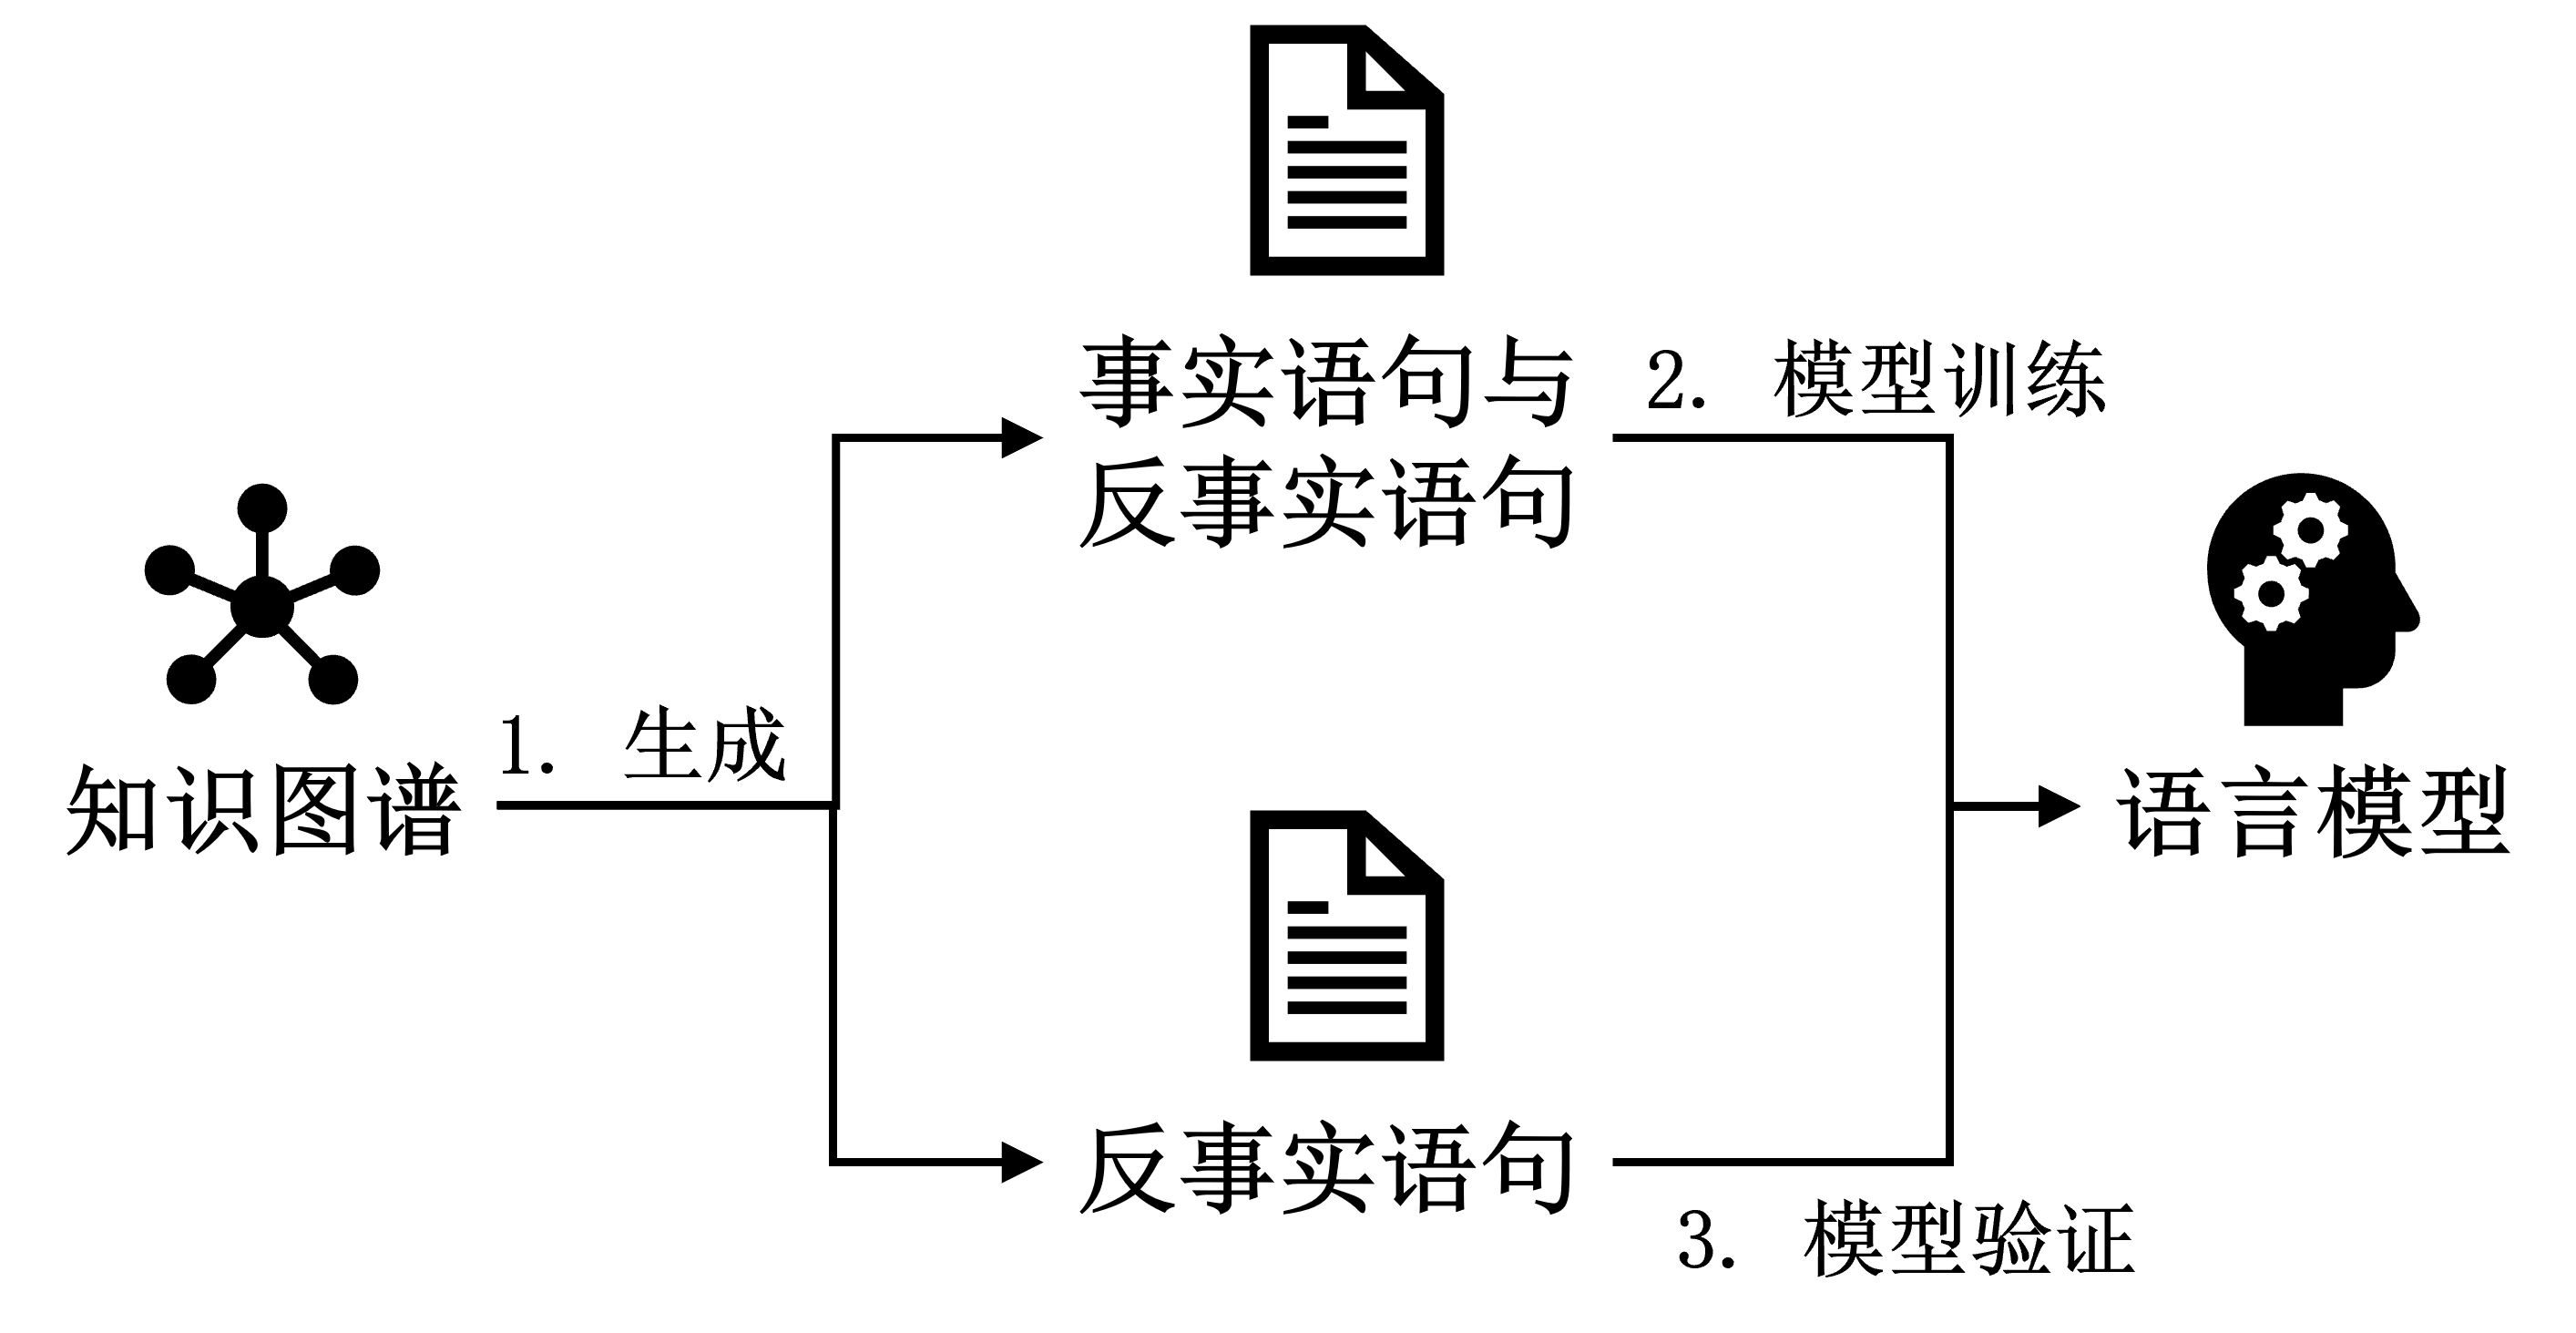
\includegraphics[width=0.5\textwidth]{images/研究方法.png}
    \caption[研究方法]{研究方法}
    \label{fig:研究方法}
\end{figure}

基于上述研究方法与具体步骤,本文将研究问题定义为三个部分,包括知识图谱选择、基于图谱的事实与反事实语句生成、以及语言模型选择。
本节将针对上述定义的三个研究问题进行说明。

\subsection{知识图谱选择}
\label{subsection:kg-selection}

由于开源知识图谱的选择众多且具有多样性,表现在知识领域、图谱规模、图谱文件类型以及数据结构等多个方面,因此选择合适的知识图谱用于事实与反实施语句生成是本文的第一个研究问题。
合适的知识图谱应包含以下几个特点:
\begin{enumerate}
    \item 以常识为知识领域,能够以常识为事实提供事实知识。
    \item 具有一定规模,能够提供支撑模型训练数据量的数据。
    \item 图谱内数据结构合理,且最好能为事实生成提供有效的额外信息。
\end{enumerate}

针对这三个特点,本文选择ConceptNet\footnote{ConceptNet:https://conceptnet.io/}作为实验知识图谱。
ConceptNet是一个免费提供的语义网络,同时也是一个知识图谱,旨在帮助计算机理解人们使用的词语的含义。
ConceptNet起源于众包项目Open Mind Common Sense,该项目于1999年在麻省理工学院媒体实验室启动。
该项目已经发展到包括来自其他众包资源的知识、专家创造的资源和有目的的游戏。
ConceptNet5版本已经包含有2800万关系描述。

相同于常规开源知识图谱,ConceptNet的原始数据集格式为CSV文件,但与此同时,ConceptNet还提供REST API 以获取 JSON-LD 格式的数据\footnote{ConceptNet web API:https://github.com/commonsense/conceptnet5/wiki/API}。
以下代码给出了使用REST API获取以实体$example$为主语的一组三元组的数据后得到的返回结果样例,同时展示了ConceptNet的数据结构。


\begin{lstlisting}[language=json,firstnumber=1]
{
    "@id": "/a/[/r/IsA/,/c/en/example/n/,/c/en/information/n/]",
    "dataset": "/d/wordnet/3.1",
    "end": {
        "@id": "/c/en/information/n",
        "label": "information",
        "language": "en",
        "sense_label": "n",
        "term": "/c/en/information"
    },
    "license": "cc:by/4.0",
    "rel": {
        "@id": "/r/IsA",
        "label": "IsA"
    },
    "sources": [
        {
            "@id": "/s/resource/wordnet/rdf/3.1",
            "contributor": "/s/resource/wordnet/rdf/3.1"
        }
    ],
    "start": {
        "@id": "/c/en/example/n",
        "label": "example",
        "language": "en",
        "sense_label": "n",
        "term": "/c/en/example"
    },
    "surfaceText": "[[example]] is a type of [[information]]",
    "weight": 2.0
}
\end{lstlisting}

可以观察到,返回的JSON数据中除去构成三元组的包含4-10行、22-28行的实体信息以及12-15行的关系信息外,同时还提供的$surfaceText$与$weight$信息。
一些ConceptNet的数据是从自然语言文本中提取的,$surfaceText$的值展示提取这个数据的原始文本是什么,而$weight$值显示这个信息有多可信,当信息来自更多的来源或更可靠的来源时,$weight$值会更高。


\subsection{基于图谱的反事实语句生成}
基于小节~\ref{subsection:kg-selection}选择的知识图谱,本小节给出事实与反事实语句生成的具体方法。
本文定义能从所选知识图谱中获取到的知识为事实,而无法通过图谱内知识验证其正确性的知识为反事实。
由于ConceptNet为多数三元组通过键$surfaceText$提供了该三元组所表示的事实的自然语言描述文本,因此本小节主要阐述反事实与反事实语句的生成方法。

反事实三元组生成的方法主要通过限定关系的三元组实体替换来实现,具体方法为随机选择一种关系,并在图谱中选择两个以该关系组成的三元组,且这两个三元组满足包含的四个实体各不相同的条件。
针对这两个三元组,对主语实体或宾语实体进行替换,且在图谱中寻找是否存在替换后的三元组。基于上述的反事实定义,若不存在,则认定该三元组为反事实三元组。
通过限定关系的实体替换反事实三元组生成方法,获得的反事实三元组在保证语义的同时,也能获取有意义的知识信息。

基于上述反事实三元组,本文根据三元组关系的自然语言模板进行反事实语句生成。
具体而言,由于ConceptNet为每一个三元组提供了自然语言表示,模板与关系的映射也由此确定了。
因此可以根据反事实三元组与关系模板构建反事实语句。

\subsection{语言模型选择}

\subsubsection{ALBERT}
BERT等预训练语言模型出现以来,都采用了很大的参数量以取得更好的效果。ALBERT模型的动机是基于这样一个认识:模型参数量越来越大也带来了很多问题,比如对算力要求越来越高、模型需要更长的时间去训练、甚至有些情况下参数量更大的模型表现却更差。作者做实验发现,将BERT-large的隐藏层参数量翻倍得到BERT-xlarge模型,两者比较发现BERT-xlarge虽然有更多的参数,但是在预训练阶段其损失函数的值波动比BERT-large更大,在数据集RACE上的表现远远低于BERT-large。为了解决参数量过大的问题,提出了两种减少预训练模型参数的方法:分解嵌入参数化和跨层参数共享。此外,还提出使用句序预测(SOP)任务代替原始BERT中的下一句预测(NSP)任务。
\paragraph{分解嵌入参数}
在BERT、XLNet等模型中词向量的大小总是与隐藏层大小相同,如果每个词向量都与隐藏层大小一致,将会导致模型参数量过大。因此可以通过减少嵌入层的词向量维数,ALBERT的提出者认为,词向量只是记忆了相对少量的词语的信息,更多的语义和句法等信息时由隐藏层记忆的。因此,词嵌入的维度可以不必与隐藏层的维度一致,可以通过降低词嵌入的维度的方式来减少参数量。
\paragraph{跨层参数共享}
第二个减少参数量的方法是隐藏层的参数共享,即多个层之间的参数一致,反向传播时只更新一次。在ALBERT中,参数共享的方式有三种:1)只共享全连接层的参数,2)只共享注意力层的参数,3)全连接层、注意力层的参数均共享。默认情况下是第三种方式,这样就大大减少模型的参数量。
\paragraph{句序预测(SOP)}
在BERT中,句子间关系的任务是下一句预测(NSP),随机将两个句子中的下一个句子替换成另一个句子,预测第二个句子是不是第一个句子的下一句,是一个二元分类。

在ALBERT中,对BERT的NSP任务进行改进,其任务叫做句序预测(SOP),即句子间顺序预测。给定模型两个句子,让模型去预测两个句子的前后顺序,相当于正例和NSP一致,即原来的句子顺序。而负例中,NSP是随机替换第二个句子为另一个句子,SOP是对同一个数据中两个句子交换顺序。SOP是比NSP要更为复杂的任务,因为SOP的负例还是在同一篇文档中得到,他们拥有共同的主题,预测的是句子间的连贯性。因此相比于NSP,通过SOP任务模型能够学到更多的句子间的语义关系。

\subsubsection{XLNet}
XLNet模型是一种大规模预训练语言模型,针对于BERT模型几个缺点进行改进,在SQuAD、GLUE、RACE等20个任务上全面超越BERT。BERT训练时将部分单词mask起来,使模型能够利用句子双向的信息,在很多NLU任务上取得很好的效果。然而,由于需要mask一部分输入,BERT忽略了被mask位置之间的依赖关系,并且微调过程与预训练过程不一致,找成了这两个过程效果之间的差异。

基于这些优缺点,提出了一种泛化的自回归预训练模型XLNet。XLNet可以:1)通过最大化所有可能的顺序的对数似然,学习双向语境信息;2)用自回归本身的特点克服BERT的缺点。此外,XLNet还融合了当前最优自回归模型Transformer-XL的思路。

首先介绍一下预训练模型中的自回归(Auto Regression, AR)模型与自编码(Auto Encoder, AE)模型。AR模型简单来说就是用序列中t时刻的token作为输出,那么这个token之前(1至t-1时刻)所有token组成的序列作为输入来预测t时刻的token。这样建模有一个缺点就是只能用前面的信息预测后面,而后面的信息对预测没有任何作用。并且这种缺点是不能用双向预测然后拼接来得到解决的,因为双向预测中,每一向还是和AR模型一样。这样忽略了上下文信息,导致预测不是很准确。AE模型是随机mask掉序列数据中某些token,得到一个新的序列数据,用该序列去预测那些被mask掉的值。这样的好处是利用了整个序列的信息去预测某些被mask的值,利用了上下文信息。但是坏处是预训练阶段和微调阶段不一致。

AR的方法可以更好地学习token之间的依赖关系,而AE的方法可以更好地利用深层的双向信息。XLNet结合AR模型和AE模型的优点,采用了置换语言模型 (Permutation Language Model, PLM),将句子随机排列,然后用自回归的方法训练,从而获得双向信息并且可以学习token之间的依赖关系。如下图所示,PLM将原始序列随机打乱顺序,例如原始序列为“123456”,打乱得到一个序列“542631”,那么将末尾的词mask一部分,在这个新得到的打乱的序列应用自回归模型来计算末尾被mask的值。因为序列被打乱了,那么后面的信息就会出现在前面,例如要预测“3”,在原始序列中“3”之后的token“4”“5”“6”就出现在前面,就利用了整个上下文的信息,这属于AE的思路。然后打乱序列利用AR的思路预测,这样就结合了AR和AE的优点。

\begin{figure}[htb]
    \centering
    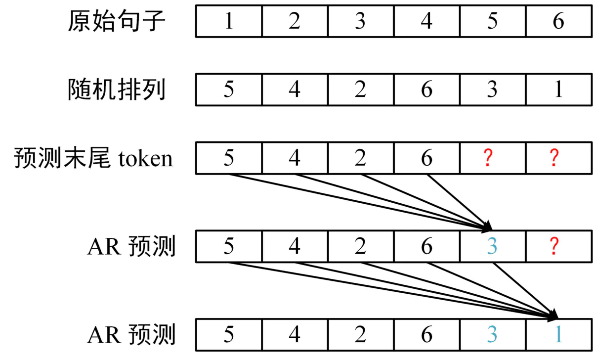
\includegraphics[width=0.5\textwidth]{images/xlnet.png}
    \caption[xlnet]{XLNet的PLM}
    \label{fig:xlnet}
\end{figure}

XLNet的核心思想就是PLM,在实践中还使用了Transformer-XL的优化方式,该优化方式是为了解决捕获长期依赖时梯度存储内存爆炸的问题。
